\chapter{Autentificación por credenciales VPN}
\label{anexo:a}
El script PiVPN  generará y gestionará los certificados tanto de los clientes como del servidor. Con el archivo ovpn generado se le dará al cliente su par de claves y la clave pública del servidor. En el momento de la conexión, tanto el cliente como el servidor usarán los datos que poseen para generar la conexión segura.

\begin{figure}[H]
  \centering
  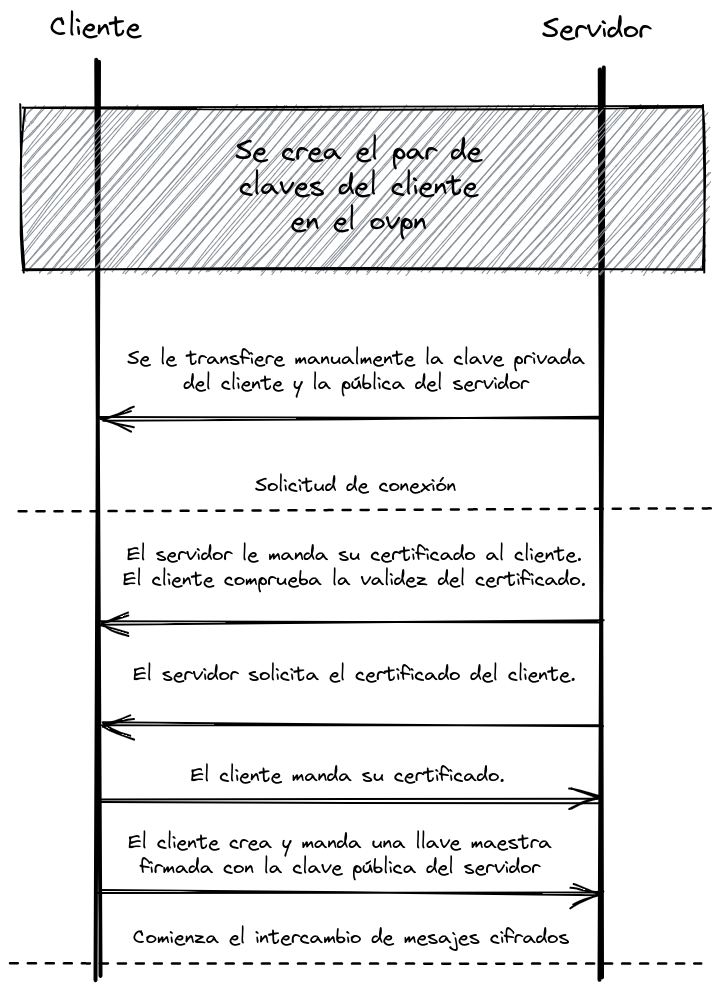
\includegraphics[width=0.6\textwidth]{figura4.png}
  \caption{Proceso de inicio de conexión VPN}
  \label{fig:SSLHandshake}
\end{figure}